%%%%%%%%%%%%%%%%%%%%%%%VICARIOUS%%%%%%%%%%%%%%%%%%%%%%%%%%%%%%%%%%%%%%%
% 																	%
% Template for presentation in Latex`s Beamer Class					%
% Using the default Berlin theme, can be replaced by other themes		%
% logo in the upper right can be replaced by new .png, gif, eps etc	%
% 																	%
%%%%%%%%%%%%%%%%%%%%%%%%%%%%%%%%%%%%%%%%%%%%%%%%%%%%%%%%%%%%%%%%%%%%%%%
\documentclass[xcolor=dvipsnames, aspectratio=169]{beamer}
\usetheme{Berlin}
\usecolortheme[named=LimeGreen]{structure}
\usepackage{beamerthemesplit} % kam neu dazu
\usepackage[ngerman]	{babel}			
\usepackage{t1enc}						
\usepackage[utf8]{inputenc}			
\usepackage{amsmath}
\usepackage{graphicx}
\graphicspath{{pictures/}}
\usepackage{amssymb}
\usepackage{amsfonts}
\usepackage{caption}
\usepackage{multimedia}
\usepackage{tikz}
\usepackage{listings}
\usepackage{acronym}
\usepackage{subfig}

\usepackage{lmodern}
\usepackage{multicol}

\definecolor{pblue}{rgb}{0.13,0.13,1}
\definecolor{pgreen}{rgb}{0,0.5,0}
\definecolor{pred}{rgb}{0.9,0,0}
\definecolor{pgrey}{rgb}{0.46,0.45,0.48}

\lstset{
    escapeinside={(*}{*)}
}


\lstdefinestyle{basic}{  
  basicstyle=\footnotesize\ttfamily,
  breaklines=true
  numbers=left,
  numberstyle=\tiny\color{gray}\ttfamily,
  numbersep=7pt,
  backgroundcolor=\color{white},
  showspaces=false,
  showstringspaces=false,
  showtabs=false,
  frame=single,
  rulecolor=\color{black},
  captionpos=b,
  keywordstyle=\color{blue}\bf,
  commentstyle=\color{gray},
  stringstyle=\color{green},
  keywordstyle={[2]\color{red}\bf},
}


\lstdefinelanguage{custom}
{
morekeywords={public, void},
sensitive=false,
morecomment=[l]{//},
morecomment=[s]{/*}{*/},
morestring=[b]",
}


\lstdefinestyle{BashInputStyle}{
  language=bash,
  showstringspaces=false,
  basicstyle=\small\sffamily,
  numbers=left,
  numberstyle=\tiny,
  numbersep=5pt,
  frame=trlb,
  columns=fullflexible,
  backgroundcolor=\color{gray!20},
  linewidth=0.9\linewidth,
  xleftmargin=0.1\linewidth
}

%Logo in the upper right just change if you know what you are doing^^
\addtobeamertemplate{frametitle}{}{%
\begin{tikzpicture}[remember picture,overlay]
\node[anchor=north east,yshift=2pt] at (current page.north east) {
\includegraphics[height=1.8cm]{htw}};
\end{tikzpicture}}

\begin{document}
\bibliographystyle{alpha}
\title{Netzwerke -- Übung WiSe2018/19}
\subtitle{Routing Teil 2\\
		Backbone-Routing\\
		\href{mailto:Benjamin.Troester@HTW-Berlin.de}{Benjamin.Troester@HTW-Berlin.de}\\
		PGP: ADE1 3997 3D5D B25D 3F8F 0A51 A03A 3A24 978D D673 }
\author{Benjamin Tröster}

\date{}

\begin{frame}
\titlepage

\end{frame}

\section*{Road-Map}
\begin{frame}
\frametitle{Road-Map}
\begin{multicols}{2}
  \tableofcontents
\end{multicols}
\end{frame}

\section{Retrospektive}
\begin{frame}{Retrospektive}
\begin{itemize}
	\item Vorlesung
	\begin{itemize}
		\item Retrospektive der Vorlesung -- was haben Sie behandelt?
		\begin{itemize}
			\item OSI 2 -- Data Link Layer (MAC \& LLC) -- Fragen?
		\end{itemize}
		\item Übungsblatt -- Fragen?
	\end{itemize}
\end{itemize}
\end{frame}


\section{Präsentation}

\subsection{Backbone-Routing}
\begin{frame}
\frametitle{1.) Planung des Netzwerkes \& Routing}
	\begin{itemize}
		\item Diskutieren Sie anhand eines Beispiels die theoretische Umsetzung des Backbone-Netzwerkes.
		\item Erläutern Sie mithilfe einer geeigneten Skizze die Architektur Ihres Netzwerkes  samt IP-Adressen, Subnetzmaske, (Default-) Gateway(s).
		\item Erläutern Sie, wie und auf welchen Geräten Routen zu setzen sind. Wo werden \emph{Default-Gateways} und wo normale \emph{Gateways} eingesetzt?
	\end{itemize}
\end{frame}

\subsection{Tools}
\begin{frame}
	\frametitle{2.) Tools: \emph{netstat} \& \emph{ss}}
	\begin{itemize}
		\item \textbf{Wiederholung:} Erläutern Sie die Syntax, sowie die Semantik der beiden Tools \emph{ip route} und \emph{route}. (Sie können dies schrittweise durchgehen!)
		\item Erläutern Sie die Funktionen der Tools \emph{netstat} und \emph{ss}.
		\item Diskutieren Sie anhand von Beispielen, wie und wozu \emph{netstat} bzw. \emph{ss} genutzt wird.
	\end{itemize}
\end{frame}

\subsection{NAT}
\begin{frame}
	\frametitle{3.) \emph{NAT}}
	\begin{itemize}
		\item Erläutern Sie was \emph{NAT} ist und wo es zum Einsatz kommt.
		\item Erläutern Sie wie \emph{NAT} umgesetzt wird. D.h. wie werden die Pakete zugeordnet?
		\item Erklären Sie was eine Firewall im Kontext von Computernetzwerken ist.
		\item Erläutern Sie wie \emph{iptables} (als Firewall) und \emph{NAT} in unserem Labor zusammenhängen. 
	\end{itemize}
\end{frame}

\subsection{Routing-Algorithmen}
\begin{frame}
\frametitle{4.) Dijkstra-Algorithmus}
	\begin{itemize}
		\item Zeigen Sie anhand folgenden Beispiels, wie der Dijkstra-Algorithmus funktioniert.
	\end{itemize}
	\begin{figure}[H]
	\centering
	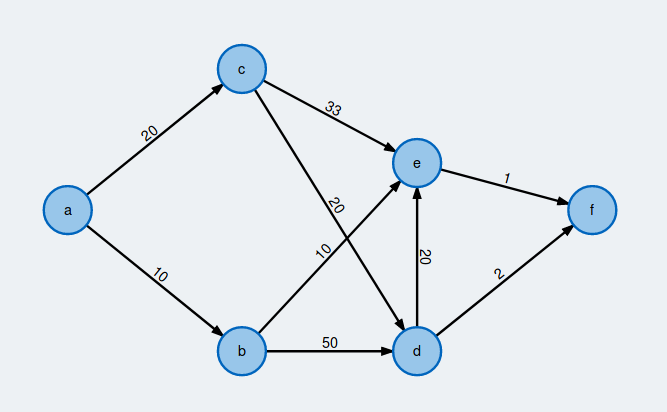
\includegraphics[scale=0.35]{dijkstra_example}
	\end{figure}
\end{frame}

\begin{frame}
\frametitle{5.) Bellman-Ford-Algorithmus}
	\begin{itemize}
		\item Zeigen Sie anhand folgenden Beispiels, wie der Bellman-Ford-Algorithmus funktioniert.
	\end{itemize}
	\begin{figure}[H]
	\centering
	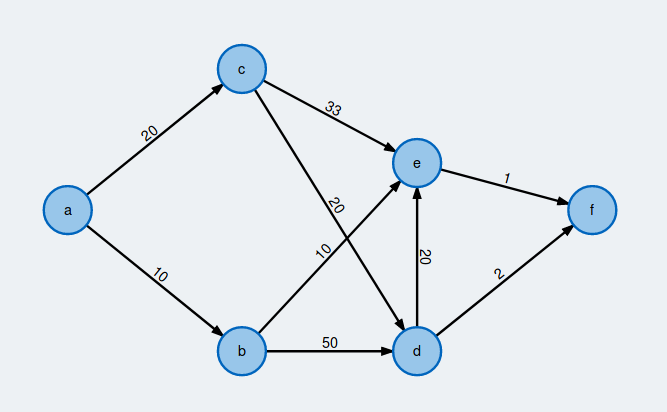
\includegraphics[scale=0.35]{dijkstra_example}
	\end{figure}
\end{frame}


\end{document}
